%!TEX root = ../Libro.tex
\section[Metodología de Desarrollo: XP]{Metodología de Desarrollo: Extreme Programming}
Extreme Programming (XP) es una metodología de desarrollo de software cuyo éxito radica en centrar los esfuerzos en la satisfacción del cliente y la mitigación de riesgos. Ésta metodología es recomendada para equipos de trabajo pequeños (de 2 a 12 desarrolladores) y hace énfasis en el trabajo en equipo. Para XP, es imperativo que el equipo de trabajo tenga a su disposición, en cualquier momento, la retroalimentación del cliente \citep{Metodologia_XP_when2006}.\\

Según \citeauthor{Metodologia_XP_whatis2006}, XP potencia los proyectos de desarrollo de software en cuatro aspectos esenciales:

\begin{itemize}
	\item \textbf{Comunicación:} existe una comunicación constante entre los clientes y los programadores.
	\item \textbf{Simplicidad:} se busca mantener un diseño simple y limpio.
	\item \textbf{Retroalimentación:} se obtiene al realizar las pruebas al software desde el primer día. Se realizan entregas parciales del sistema tan pronto como sea posible y se implementan los cambios sugeridos.
	\item \textbf{Coraje:} las características anteriores le permiten a los desarrolladores responder de forma efectiva a los cambios constantes.
\end{itemize}

\subsection{Flujo de Trabajo}
El flujo de trabajo de la metodología, como se indica en la figura \ref{fig:xp_project}, inicia con la redacción de \textbf{historias de usuario}, de las que se puede proceder a \textbf{planificar las entregas}. XP recomienda desarrollar un \textbf{esbozo de la arquitectura} que implemente de manera somera las historias de usuario que representen mayor dificultad técnica. De esta manera la estimación del tiempo de desarrollo de cada historia, durante la planificación, será más acertada \citep{Metodologia_XP_flujograma2006}. \\

\begin{figure}[ht]
	\centering
	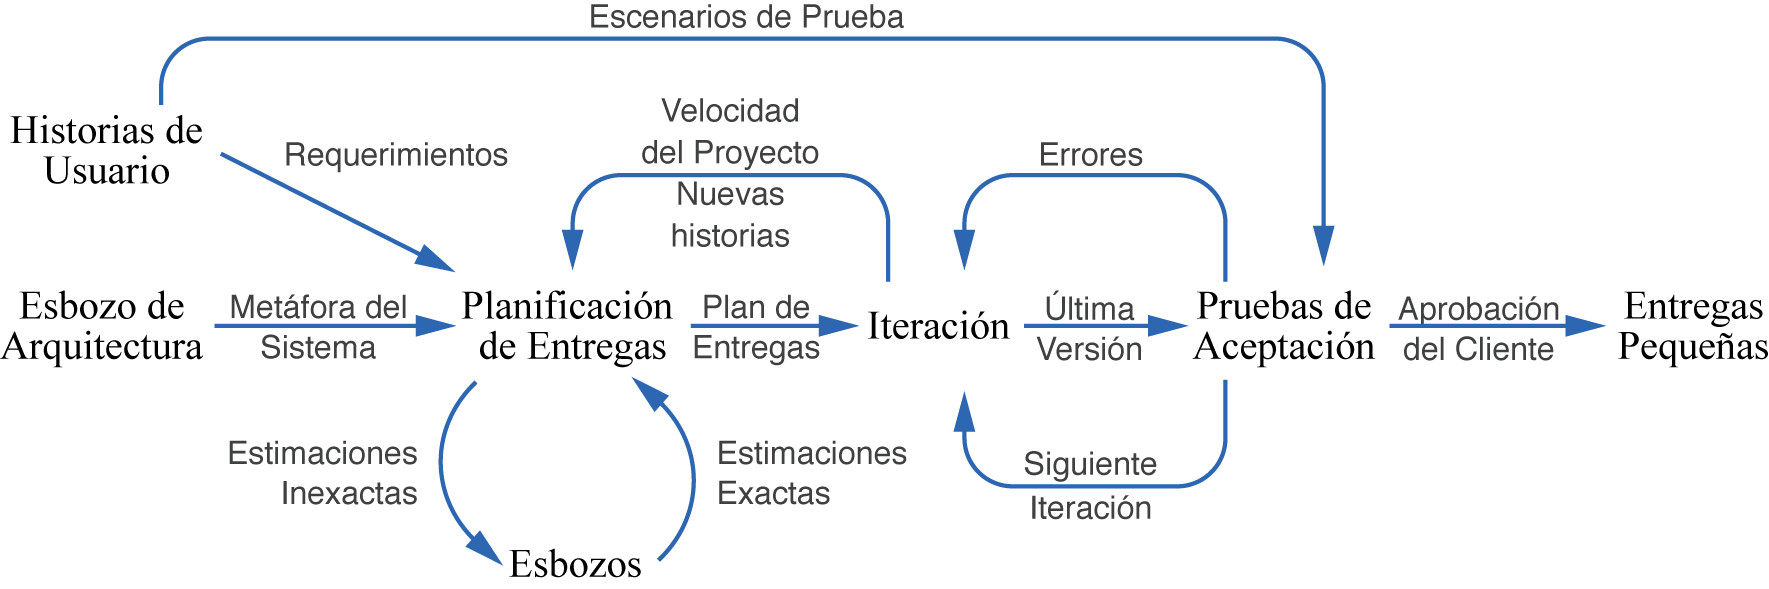
\includegraphics{imagenes/XP-Flujo.png}
	\caption{Flujo de Trabajo en Extreme Programming. \citep{Metodologia_XP_grafico_flujograma_2006}}
	\label{fig:xp_project}
\end{figure}

Una vez realizada la planificación de las entregas se procede al desarrollo iterativo en el cual el cliente selecciona las historias de usuario a desarrollar y los desarrolladores diseñan las \textbf{pruebas} correspondientes. Como resultado de una iteración se obtiene la \textbf{velocidad del proyecto} que a su vez sirve de límite para la selección de las próximas historias a desarrollar. \\

XP recomienda que se realicen \textbf{entregas pequeñas}, de manera continua, de modo que el cliente pueda ofrecer la retroalimentación necesaria.

\subsection{Etapas del Flujo de trabajo en XP}
Xtreme Programming, como lo indica la Figura \ref{fig:xp_project}, contempla varias etapas dentro del flujo de trabajo, las más destacables son:

\begin{enumerate}
	\item \textbf{Historias de usuario:} son similares a los casos de uso, sin embargo no están escritas en un lenguaje técnico dado que es el cliente el encargado de redactarlas, en aproximadamente tres oraciones, basandose en sus necesidades específicas. Deben contener un nivel de detalle razonable de modo que los desarrolladores puedan hacer las estimaciones de tiempo, de manera más acertada, para las entregas. Las historias sirven como fuente de inspiración para la creación de pruebas de aceptación automatizadas \citep{Metodologia_XP_historias2006}.
	
	\item \textbf{Selección de la metáfora del sistema:} a partir de la creación del esbozo de la arquitectura y del conocimiento de las historias de usuario se enmarca el desarrollo del proyecto en una metáfora. La selección de dicha metáfora permite que el equipo de trabajo maneje el mismo criterio, de manera consistente, para los nombres de clases y métodos. Logrando así, que los desarrolladores agilicen la tarea de determinar la existencia de alguna funcionalidad o clase. \citep{Metodologia_XP_metafora2006}

	\item \textbf{Planificación de Entregas:} previo al inicio del desarrollo en iteraciones se lleva a cabo una reunión para crear el plan de entregas. El objetivo de dicha reunión es estimar cada historia del usuario en términos de semanas de programación ideales. Una semana ideal se refiere a cuánto tiempo estima el desarollador que le tomará implementar cada historia y sus pruebas trabajando con dedicación exclusiva al proyecto. Luego de hacer las estimaciones, el cliente procede a seleccionar las historias a implementar de acuerdo a su prioridad \citep{Metodologia_XP_entregas20061} \\ La filosofía para lograr un concenso durante la reunión de planificación de entregas debe girar en torno a cuatro variables: alcance, recursos, tiempo y calidad.
	\begin{itemize}
		\item Alcance: cuánto se tiene por hacer.
		\item Recursos: cuántas personas están disponibles.
		\item Tiempo: cuándo estará listo el proyecto o la entrega.
		\item Calidad: qué tan bueno será el proyecto y que tan bien probado será.
	\end{itemize}
	De estas variables, la gerencia puede seleccionar sólo tres. Los desarrolladores manejarán la última. Por lo general la planificación resultante se mantendrá mientras la velocidad del proyecto sea estable y no surjan nuevas historias de usuario \citep{Metodologia_XP_entregas20062}.

	\item \textbf{Iteración:} una iteración se alimenta de tres fuentes de información: el plan de entregas, la velocidad del proyecto calculada en iteraciones anteriores y los errores reportados en las pruebas de aceptación. El desarrollo de una iteración en XP, contempla en sí varias fases como se describe en la figura \ref{fig:xp_iteration}:
	\begin{figure}[ht]
		\centering
		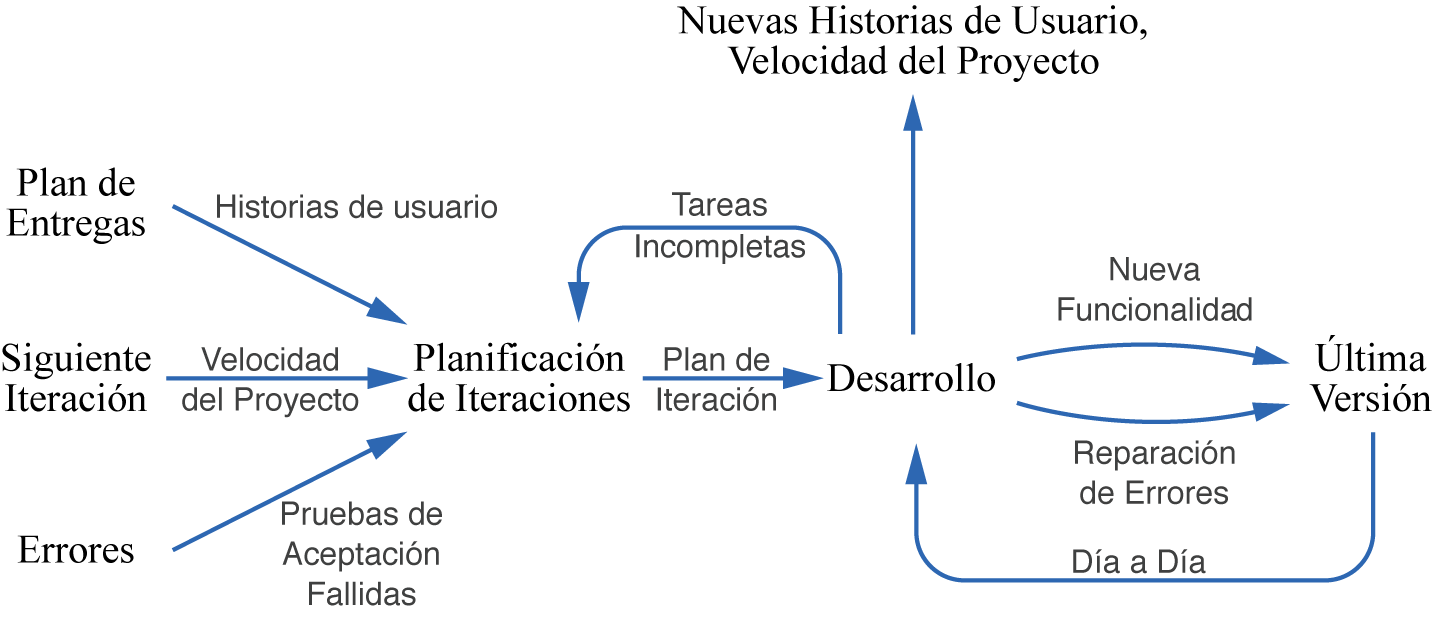
\includegraphics{imagenes/XP-Iteracion.png}
		\caption{Desarrollo iterativo - Iteración. \citep{Metodologia_XP_grafico_it_2006}}
		\label{fig:xp_iteration}
	\end{figure}

	\begin{itemize}
		\item \textbf{Planificación de iteración:} la planificación de cada iteración se realiza al principio de la misma, debe evitarse planificar por anticipado más allá de la iteración en curso, así mismo es importante mantenerse dentro de la planificación y no agregar funcionalidades que no esten planificadas. La estimación de tiempo de cada tarea debe realizarla el desarrollador asignado a dicha tarea; la estimación no debe ser modificada durante la iteración ya que de ello depende lograr mejores estimaciones en las subsiguientes iteraciones, de la misma manera debe respetarse el límite de duración de la iteración en curso \citep{Metodologia_XP_iterativo2006}.
		
		\item \textbf{Desarrollo:} el desarrollo dentro de la iteración describe un día de trabajo bajo la óptica de XP. Al inicio del día se realiza una reunión corta \citep{Metodologia_XP_standup2006} en la que se reportan problemas con sus soluciones y se promueve la concentración en el proyecto. Luego, cada desarrollador, procede a seleccionar una de las tareas asignadas (o una prueba que falle) para desarrollarla en pareja con un compañero. \\
		
		Según \citeauthor{Metodologia_XP_parejas2006}, el \textbf{desarrollo en parejas} es el punto focal del desarrollo, esta metodología promueve un mayor conocimiento del código (funcionalidades y pruebas) por parte de cada miembro del grupo. Esta forma de trabajo está rodeada de cuatro aspectos importantes: \textbf{el intercambio de parejas}  que suele ocurrir cuando alguna pareja requiere ayuda \citep{Metodologia_XP_rotacion2006}, \textbf{integración continua} de nuevo código al proyecto al desarrollar nuevas funcionalidades o pruebas unitarias \citep{Metodologia_XP_integracion2006}, \textbf{reestructuración sin piedad} (refactoring) para simplificar partes complejas del código \citep{Metodologia_XP_refactor2006} y por último \textbf{creación de pruebas unitarias} antes de desarrollar nuevas funcionalidades. \citep{Metodologia_XP_unittest2006}
	\end{itemize}
	
\item \textbf{Velocidad del proyecto}: es un indicador de cuan rápido se está desarrollando el proyecto. Se calcula a partir del número de historias de usuario (o tareas) completadas durante cada iteración. Luego se emplea para determinar cuántas y cuáles historias de usuario (o tareas) serán implementadas durante la reunión de planificación de cada iteración. También es útil cuando se desea determinar cuantas iteraciones serán necesarias para finalizar una entrega mayor \citep{Metodologia_XP_velocidad2006}.

\item \textbf{Pruebas de aceptación o funcionales}
Las pruebas de aceptación son creadas a partir de las ``historias de usuario''. En el transcurso de una iteración las ``historias de usuario'' seleccionadas en la reunión de planificación de la iteración serán traducidas a pruebas de aceptación. El cliente especifica los escenarios en los cuales se probará si una historia de usuario, que puede tener una o varias pruebas, ha sido implementada correctamente.
Las pruebas de aceptación son pruebas de caja negra al sistema, cada una de ellas representa algún resultado esperado del sistema. Los clientes son responsables de verificar la correctitud de la prueba y revisar los resultados de la misma, para así decidir cuál prueba fallida, en caso de que la haya, tiene mayor prioridad. La implementación de una historia de usuario no serán considerada completa mientras no pase todas las pruebas de aceptación asociadas a la historia \citep{Metodologia_XP_testaceptacion2006}.

\end{enumerate}

\subsection{Retroalimentación y Planificación}

La figura \ref{fig:xp_loop} muestra el ciclo donde se indican los tiempos aproximados de planificación, al igual que los tiempos en que se obtiene retroalimentación del trabajo completado.
\begin{figure}[ht]
	 \centering
	 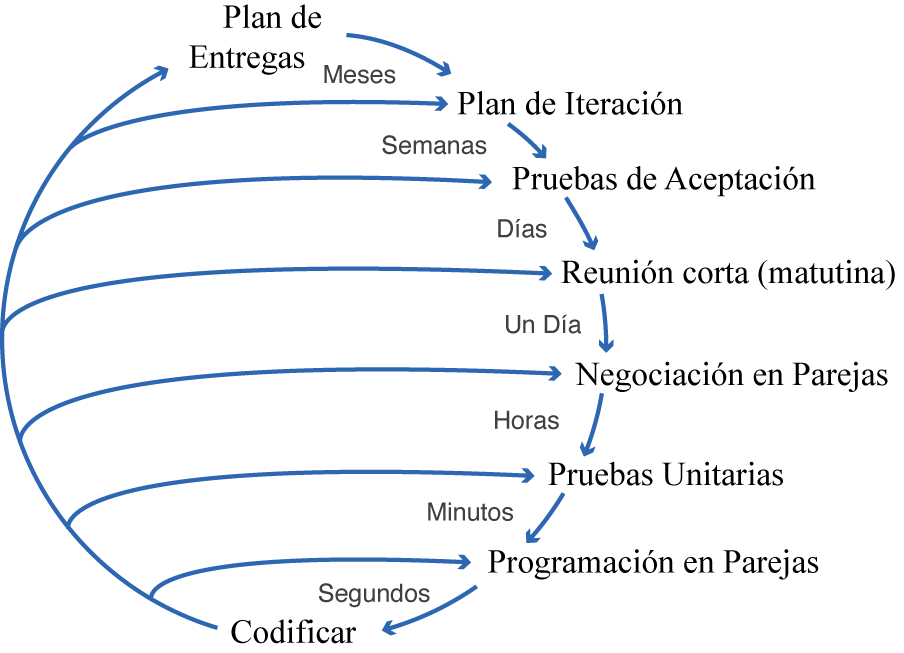
\includegraphics{imagenes/XP-feedback.png}
	 \caption{Ciclo de Planificación y Retroalimentación en Xtreme Programming}
	 \label{fig:xp_loop}
\end{figure}